\section{Semaine 21 : 26/06/2023 - 30/06/2023}
\graphicspath{{semaines/semaine_21/images/}}

\begin{abstract}
	Cette semaine, j'ai enfin compris comment faire les dérivées. En fait, Emmanuel a expliqué que le modèle est en fait une fonction et donc qu'il peut être dérivée, ainsi on connaît les dérivées de $\phi(x,y)w_\theta(x,y)$. 
	L'idée est donc de calculer les dérivées avant le passage en P10 directement avec Tensorflow puis en P10 avec FEniCS.
	
	On a également voulu tester si le problème venait de PhiFEM donc j'ai du tester la correction avec FEM.
	
	Pour finir, j'ai commencé à tester l'implémentation de la loss H1 (avec directement la dérivée par tensorflow), ça tourne mais les loss ne diminue pas.
	
	En fin de semaine, j'ai commencé à rédiger la partie sur les FNO dans le rapport. Il a également été question d'inscription à l'ED (non aboutit, en attente des résultats), j'ai donc dû faire des modifications à mon CV.
\end{abstract}

\subsection{Entraînement Loss H1}

\begin{minipage}{\linewidth}
	\centering
	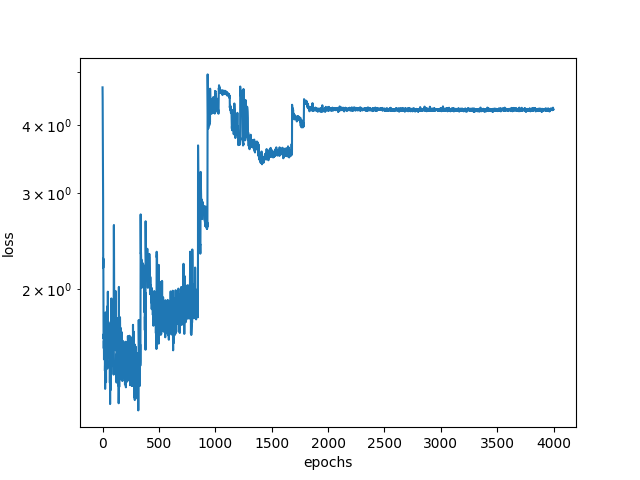
\includegraphics[width=0.35\linewidth]{history.png}
\end{minipage}

\subsection{Dérivées}

\subsubsection*{Tensorflow}

On va comparer à gauche les dérivées analytiques (calculées avec sympy), au milieu les dérivées du modèle et à droite la différence des deux. Pour le calcul de ces dérivées, on considère un échantillon de points $(x,y)$ en $\mathbb{P}^2$ avec nb\_vert=32. On utilise alors GradientTape de tensorflow pour calculer la dérivée de la prédiction du modèle (multipliée par $\phi$).

Voici les dérivées premières :

\begin{minipage}{\linewidth}
	\centering
	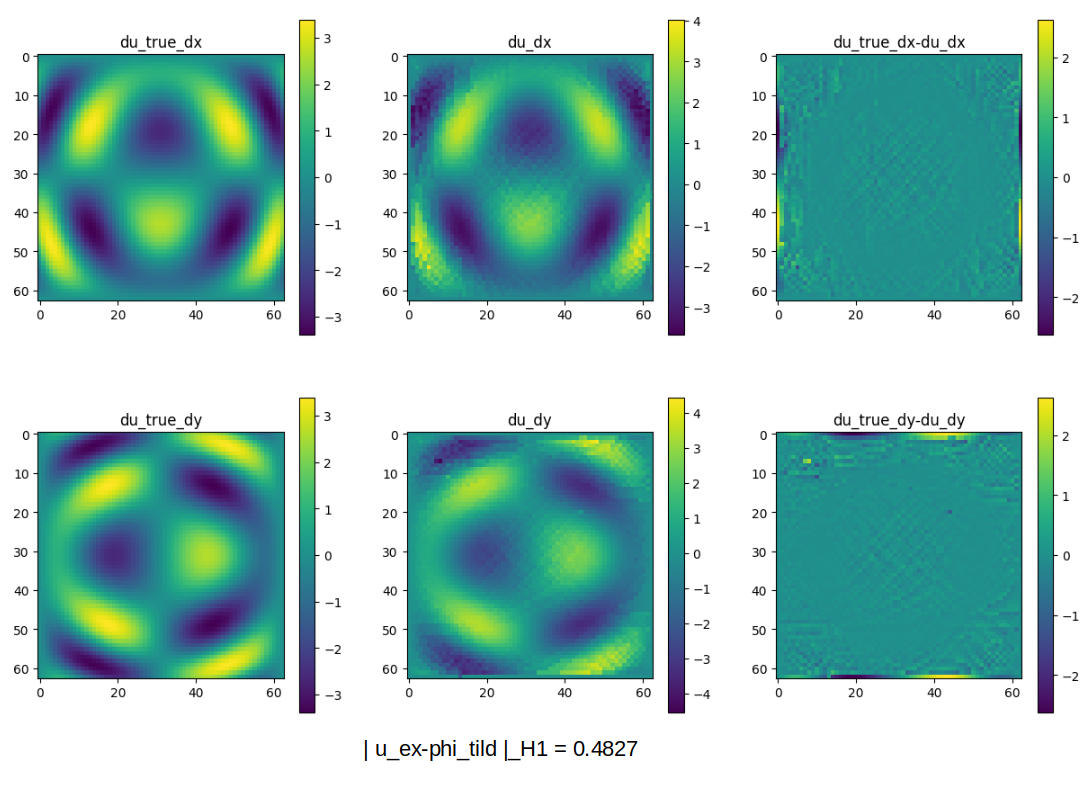
\includegraphics[width=0.75\linewidth]{Dérivées_exactes_1.png}
\end{minipage}

\newpage

Voici les dérivées secondes :

\begin{minipage}{\linewidth}
	\centering
	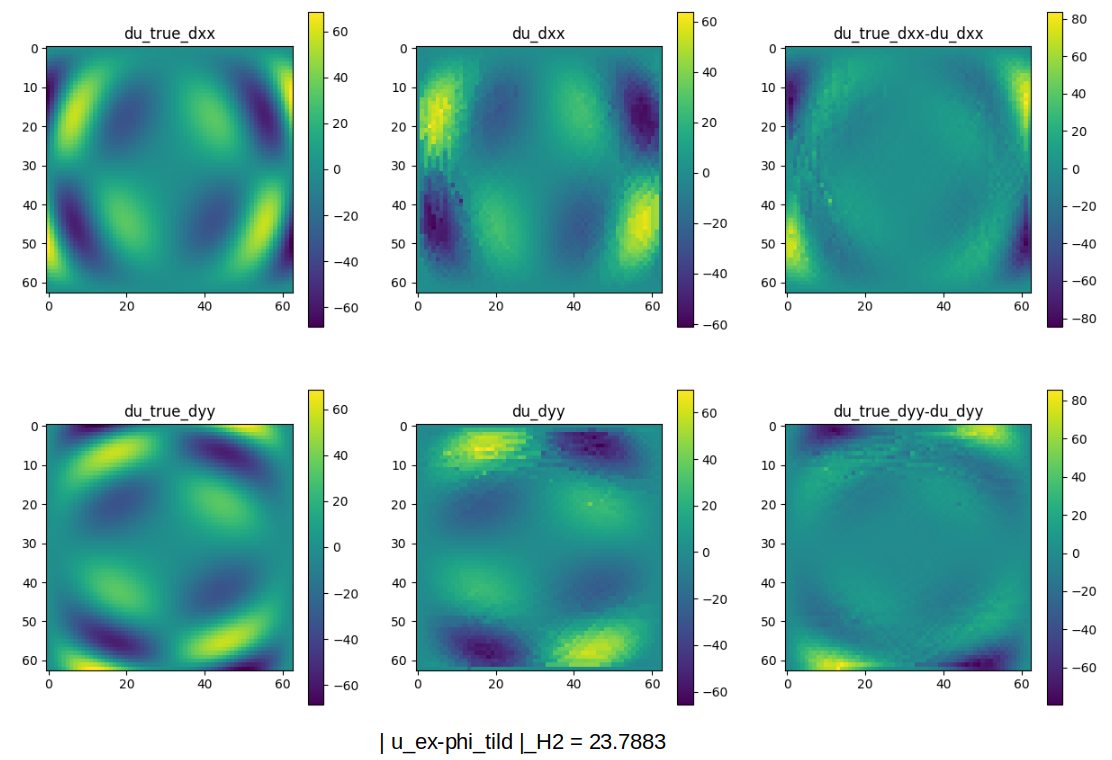
\includegraphics[width=0.75\linewidth]{Dérivées_exactes_2.png}
\end{minipage}

\subsubsection*{FEniCS}

Ici on considère du $\mathbb{P}^{10}$ avec nb\_vert=32. On ne s'intéressera ici qu'au dérivée première. A gauche, la solution analytique (avec expression FEniCS) et à droite les dérivées calculés avec la fonction grad de FEniCS.

\begin{minipage}{\linewidth}
	\centering
	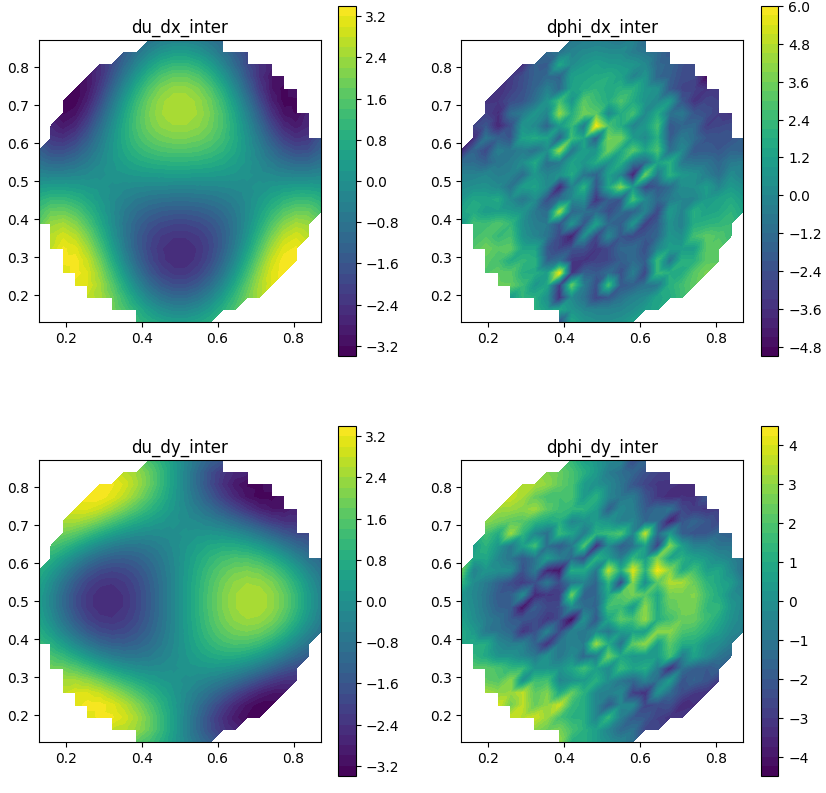
\includegraphics[width=0.65\linewidth]{Dérivées_FEniCS_1.png}
\end{minipage}

\subsection{Comparaison FEM-PhiFEM}

\begin{minipage}{\linewidth}
	\centering
	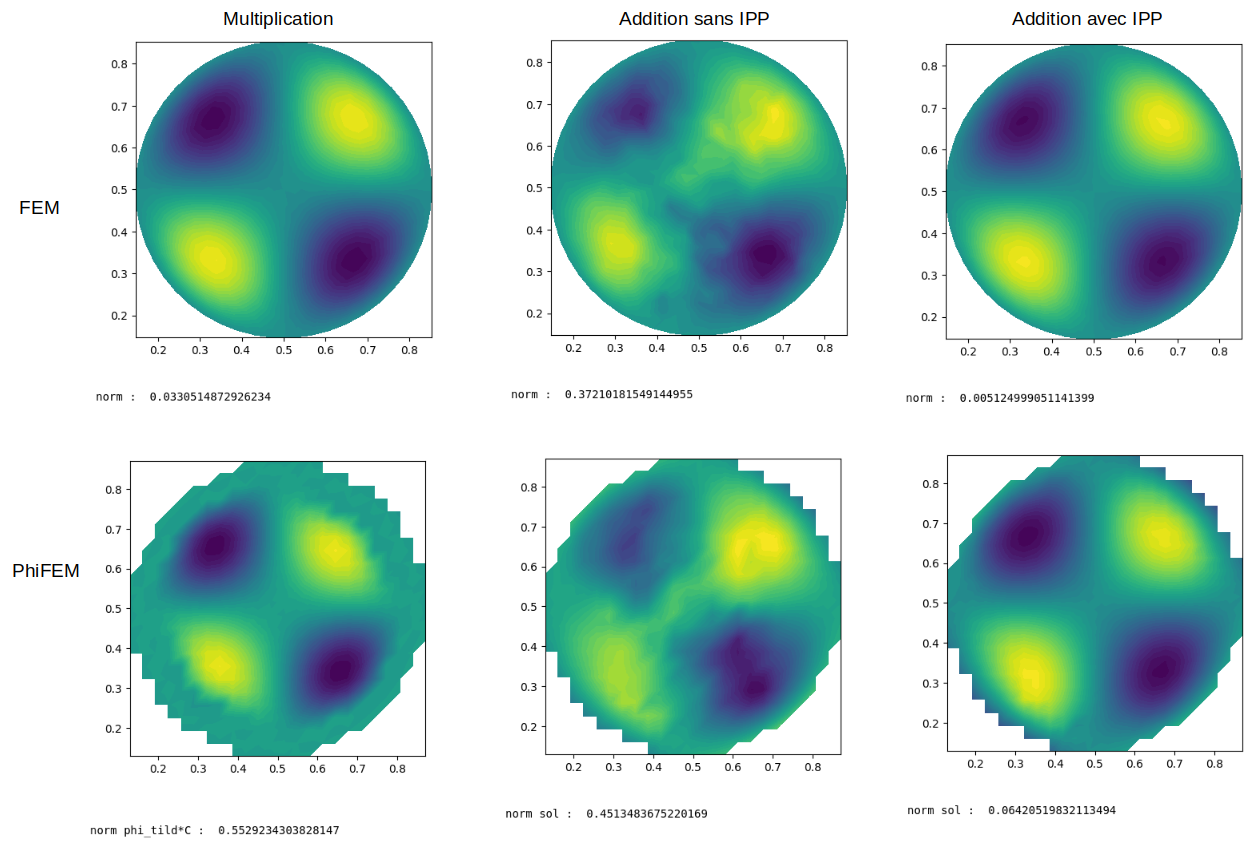
\includegraphics[width=0.9\linewidth]{FEM_vs_PhiFEM.png}
\end{minipage}

Il semblerait que la correction avec FEM fonctionne mieux qu'avec PhiFEM mais on obtient quand même pas les résultats attendus.